\documentclass[10pt,twoside]{article}
\usepackage[T1]{fontenc}
\usepackage[a4paper,margin=1in]{geometry}

% --- math ---
\usepackage{amsmath}
\usepackage{amssymb}

% --- colour, hyperlinks ---
\usepackage[dvipsnames]{xcolor}
\definecolor{codebg}{RGB}{248,248,248}
\definecolor{rulecol}{RGB}{200,200,200}
\definecolor{accent}{RGB}{0,60,120}
\usepackage[colorlinks=true,linkcolor=accent,urlcolor=accent,citecolor=accent]{hyperref}
\usepackage{graphicx}
\graphicspath{{docs/diagrams/}{diagrams/}}
\usepackage[nameinlink]{cleveref}
\crefname{lstlisting}{listing}{listings}
\Crefname{lstlisting}{Listing}{Listings}

% --- tables ---
\usepackage{booktabs}
\usepackage{multirow}
\usepackage{array}
\usepackage{tabularx}

% --- code ---
\usepackage{listings}
\lstdefinestyle{kernelh}{
  basicstyle=\ttfamily\footnotesize,
  backgroundcolor=\color{codebg},
  frame=single,
  rulecolor=\color{rulecol},
  breaklines=true,
  columns=fullflexible,
  keepspaces=true,
  showstringspaces=false,
  aboveskip=6pt,
  belowskip=6pt,
  xleftmargin=4pt,
  xrightmargin=4pt,
  tabsize=2,
}
\lstset{style=kernelh}

% --- floats ---
\usepackage{float}
\usepackage{caption}
\captionsetup{font=small,labelfont=bf}

% --- TikZ / PGFPlots ---
\usepackage{tikz}
\usetikzlibrary{arrows.meta,positioning,shapes.geometric,calc,fit,backgrounds}
\usepackage{tikz-cd}
\usepackage{pgfplots}
\pgfplotsset{compat=1.18}
\usetikzlibrary{patterns}

% --- typography ---
\usepackage[expansion=false,protrusion=true]{microtype}
\usepackage{parskip}
\usepackage{tikzflora}
\florasetup{layout=split, seed=11, density=0.55, visitors=0,
  mix={bloom=0.4, leaves=0.7, leaflets=0.5, sprays=0.3, curls=0.2,
       umbel=0, cyme=0, gyps=0, soft=0, lily=0, ghost=0}}

% --- bibliography (biber) ---
\usepackage[backend=biber,style=numeric,sorting=none,url=true,doi=true]{biblatex}
\addbibresource{references.bib}

\newcommand{\ms}{\text{ms}}
\newcommand{\gflops}{\,\text{GFLOPS}}
\newcommand{\gbs}{\,\text{GB/s}}

\title{\textbf{kernel.h}: A Cross-Vendor GPU Kernel Compiler from a C++23 DSL through Structured SSA and MLIR to NVVM/ROCDL}
\author{kernel.h project}
\date{October 2026}

\begin{document}
\pagestyle{empty}

\newgeometry{inner=2.2cm,outer=5.2cm,top=3.2cm,bottom=3.2cm,headheight=14pt,headsep=16pt}
\florathispage{layout=title}
\maketitle

\begin{abstract}
\noindent
\texttt{kernel.h} is a GPU kernel compiler. It takes one kernel description in a C++23
embedded DSL, lowers it through a custom structured-SSA IR called atom, runs a seven-pass
pipeline, lowers to an out-of-tree MLIR dialect, and emits native code for two vendors: PTX
and cubin for NVIDIA sm\_80, and AMDGCN ISA and HSACO for AMD gfx1101. The compiler uses MLIR
(LLVM 21.1.8) for the atom dialect, the \texttt{gpu}/\texttt{scf}/\texttt{vector} conversion,
and the vendor serializers. The DSL, atom IR, and the seven passes use only the project's C++
code. A thin HIP runtime loads the code objects with \texttt{hipModuleLoadData}, launches
kernels at the device ABI, and packs memref descriptors into launch arguments. A second
backend binds the CUDA Driver API at runtime with \texttt{dlopen}. The report covers the IR
design (D10), the pass pipeline with before and after dumps, the device-only lowering, the
vendor serializers, the autotuner and a correctness bug its numeric gate caught, and
measurements on an AMD Radeon RX 7800 XT (gfx1101): 347.8\,GB/s DRAM, 15\,559.8\,GFLOPS FMA,
1072.5\,GFLOPS GEMM at $8192^3$ (about 9.5$\times$ below rocBLAS), 1110\,GB/s fused GELU,
and 43.6\,GFLOPS attention. It also records the limits: tensor cores are out of scope, shared
memory is static, the GEMM has no double buffering, and the NVIDIA path is cross-compiled
locally and was run on an RTX 6000 Ada pod.
\end{abstract}
\thispagestyle{empty}

\clearpage
\thispagestyle{empty}
\newgeometry{left=3.6cm,right=3.6cm,top=3.6cm,bottom=3.6cm}
\florasetup{layout=surround}
\tableofcontents
\clearpage
\restoregeometry
\floraoff
\pagestyle{plain}

\section{Introduction and System Architecture}
\label{sec:intro}

\subsection{Goals and Scope}
\label{sec:goals}

\texttt{kernel.h} compiles one kernel description into NVIDIA and AMD GPU machine code, runs
it on the local AMD card, checks the output against an fp64 CPU reference, and benchmarks it
against AMD's vendor library (rocBLAS). The compiler uses MLIR (\cite{mlir2021}, LLVM 21.1.8)
for the atom dialect, the \texttt{gpu}/\texttt{scf}/\texttt{vector} conversion, and the
vendor serializers. The DSL, atom IR, and the seven passes are C++ code with no MLIR
dependency (\S\ref{sec:ir}).

Two compile entry points exist, both run in-process:
\begin{itemize}
  \item \texttt{kernelh-opt}: the debug and test driver. It parses \texttt{.atom} text, runs
        passes, prints IR, and provides an \texttt{mlir-opt}-style tool with the atom dialect
        registered.
  \item \texttt{kernelh}: the production CLI. Its subcommands are \texttt{compile},
        \texttt{explore}, \texttt{bench}, and \texttt{tune}. It links the DSL, IR, passes,
        emitter, backends, and runtime in-process.
\end{itemize}

\subsection{Architecture Overview}
\label{sec:arch}

The toolchain is shown in \cref{fig:arch}. A kernel description flows from the C++23 DSL
builder through atom, the seven-pass pipeline, the atom MLIR dialect, and the
\texttt{gpu}/\texttt{scf}/\texttt{vector} device module to the NVVM/ROCDL serializers. The
runtime loads the resulting HSACO or cubin through the HIP module loader or the
\texttt{dlopen}ed CUDA Driver API backend and launches it on the GPU. End-to-end tests compare
the output against an fp64 reference, and the benchmark harness compares it against rocBLAS.

\begin{figure}[H]
\centering
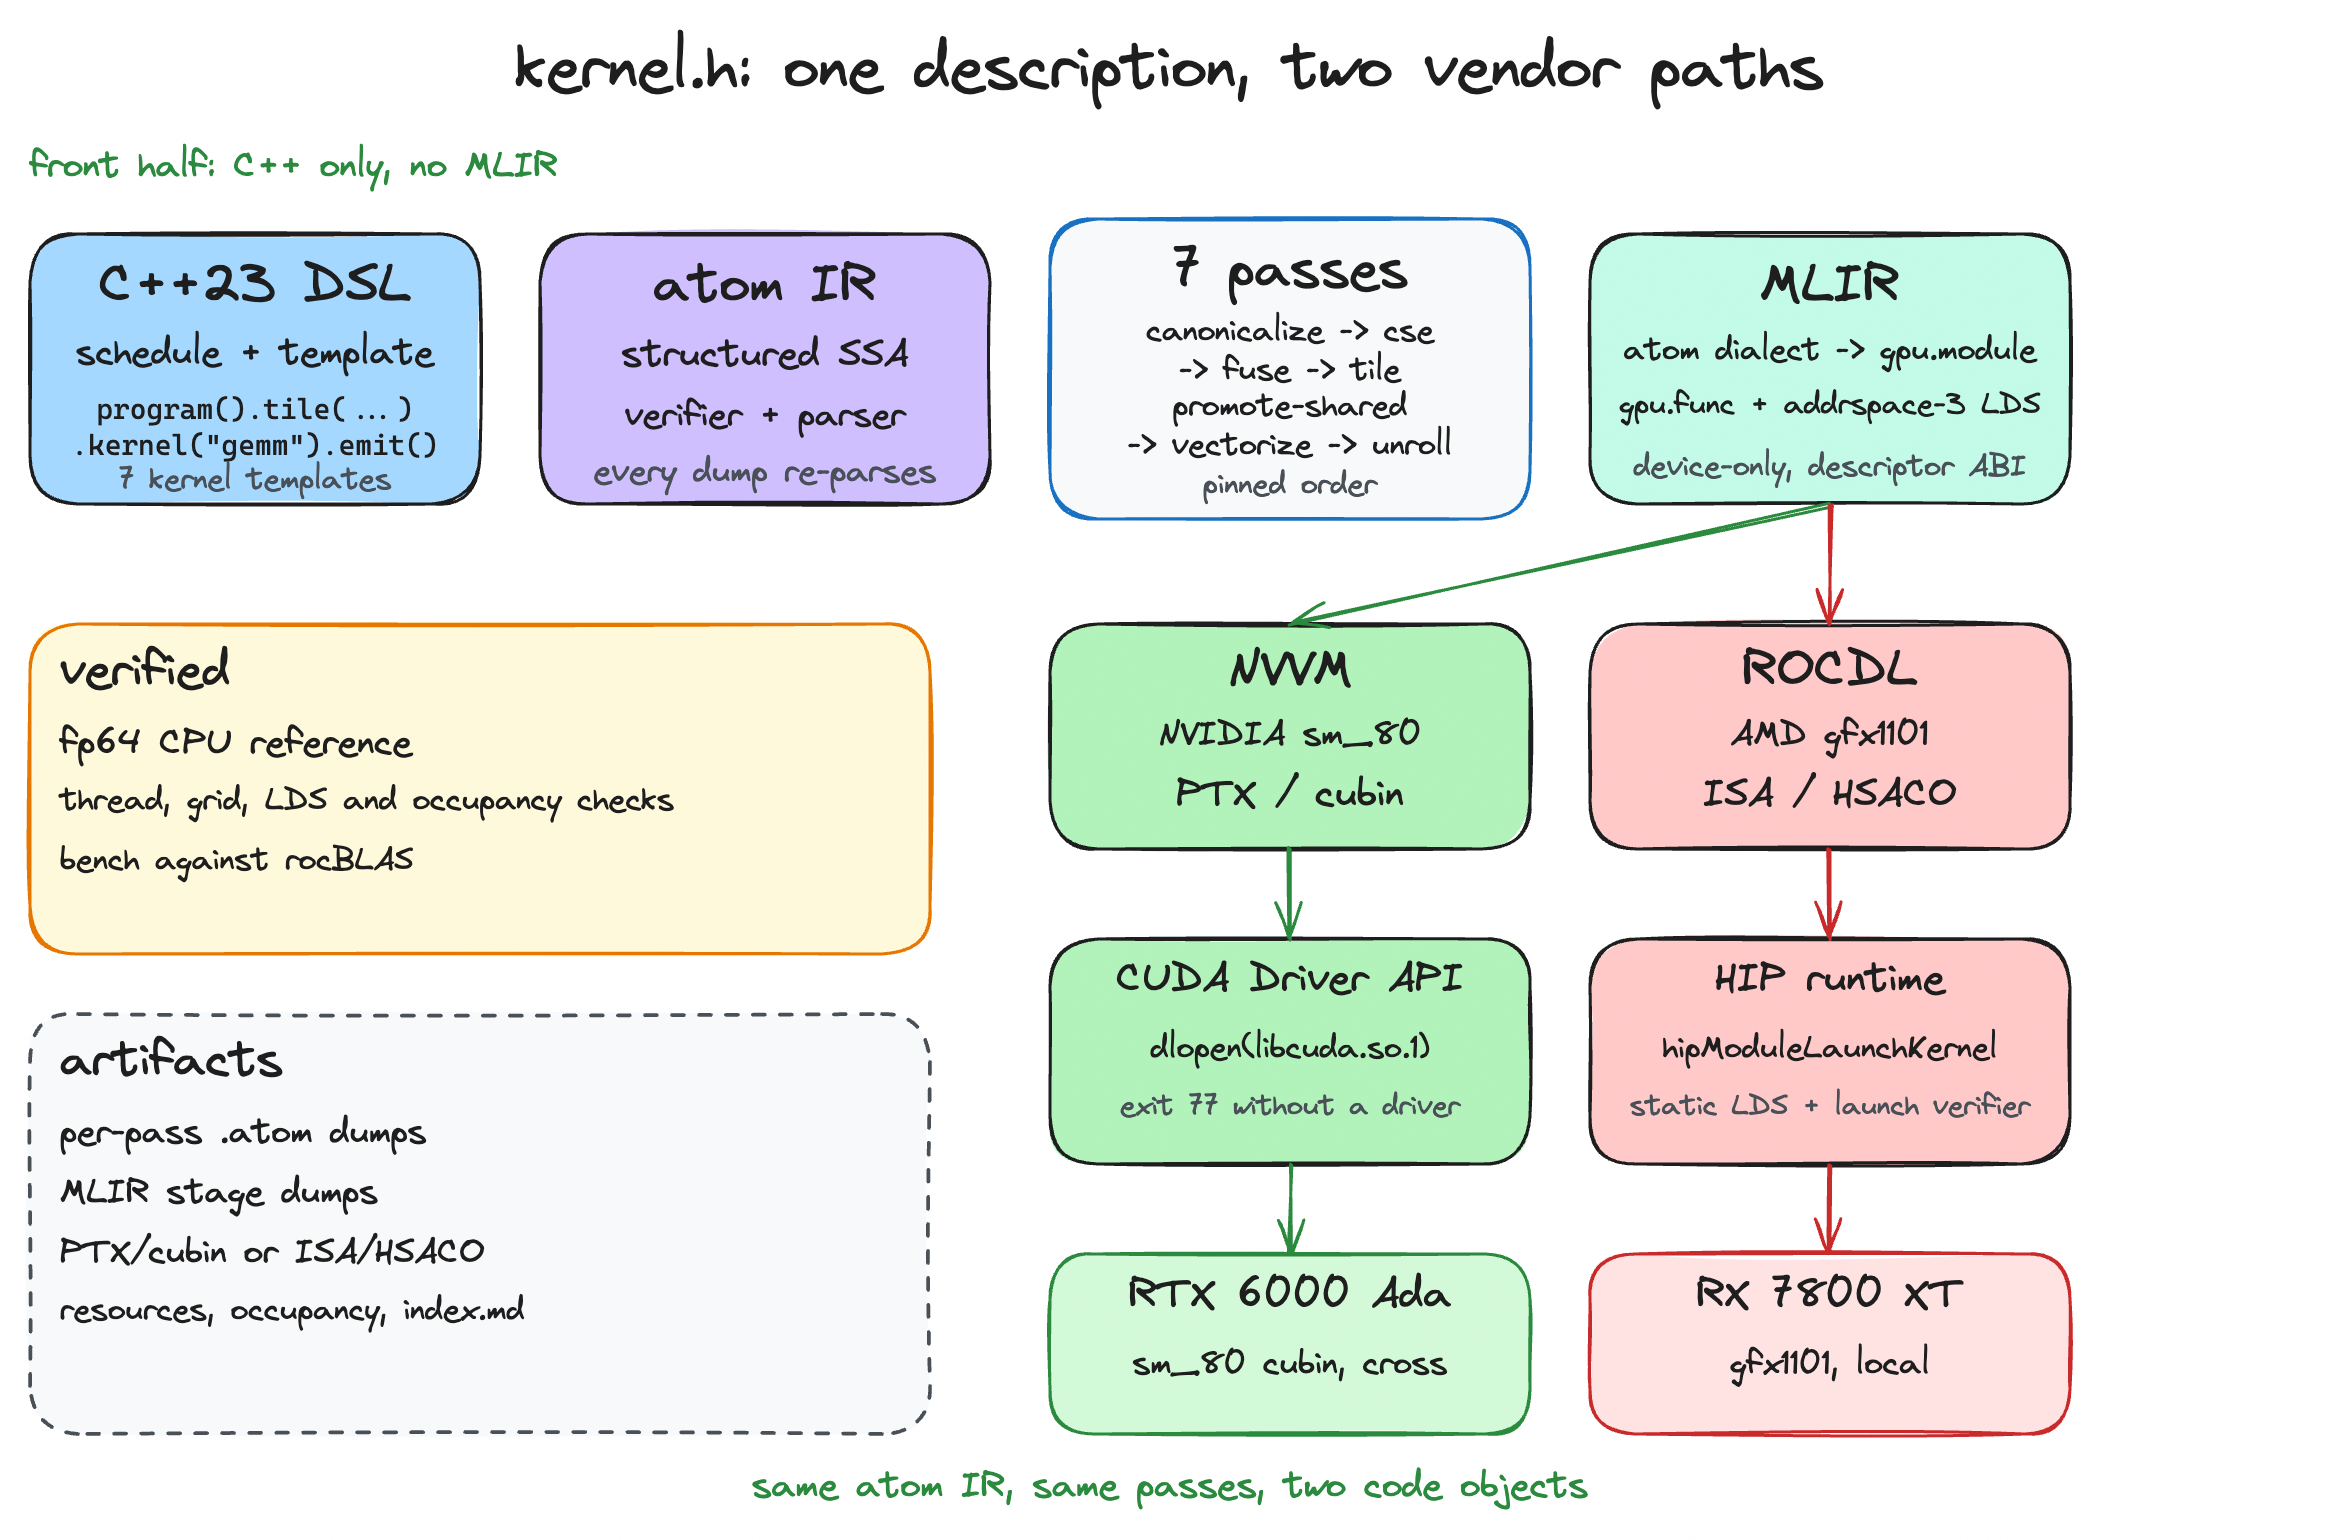
\includegraphics[width=\textwidth]{report-architecture.png}
\caption{End-to-end architecture of \texttt{kernel.h}. A kernel description flows from the
C++23 DSL through atom IR and the seven passes to the atom MLIR dialect and the
\texttt{gpu}/\texttt{scf}/\texttt{vector} device module. NVVM and ROCDL serialize the module
to PTX/cubin and ISA/HSACO. The runtime loads either code object and launches it on the GPU.
The left panels list the checks and artifacts that accompany the compile path.}
\label{fig:arch}
\end{figure}

The host measurement platform is the AMD Radeon RX 7800 XT (gfx1101, Navi 32): 30 compute
units, 16\,GiB VRAM (17\,163\,091\,968 bytes), 64\,KiB LDS per workgroup, and wavefront size
32. It runs in full runtime mode (\texttt{degraded=false}, \S\ref{sec:validation}).

\section{IR Design: Structured SSA}
\label{sec:ir}

\subsection{Rationale (decision D10)}
\label{sec:d10}

The atom IR is \emph{structured SSA}: nested block scopes with values dominating within their
scope. Control flow uses \texttt{atom.loop\_for} with
\texttt{iter\_args() -> (...)}. The loop is a structured loop and the only SSA merge point;
loop-carried values are its iter\_args, terminated by \texttt{atom.yield}.
\texttt{atom.reduce} (sum or max over a tensor dim) is built on \texttt{loop\_for} and
iter\_args.

Three properties drive the design:
\begin{enumerate}
  \item \textbf{Reductions stay in the IR.} Softmax's running max and sum, GEMM's accumulator,
        scan's carry, and attention's online statistics are loop-carried iter\_args. They
        need no conversion to a generic CFG. The pass pipeline, fusion in particular, inspects
        loop domains and barriers. A structured form makes ``same iteration domain, same
        barrier state'' a local check.
  \item \textbf{The verifier is structural.} Dominance, barrier placement, operand types, and
        shared-memory totals are structural properties. \texttt{verifyModule} reports every
        violation in one pass; it collects all diagnostics and does not stop at the first. The
        round-trip self-check in \texttt{kernelh explore} uses this (\S\ref{sec:pipeline}).
  \item \textbf{The text round-trips.} \texttt{.atom} is both printer output and parser input.
        A deterministic value-numbering scheme (an MLIR-style active-name set, where nested
        scopes do not shadow a live outer name) makes every per-pass dump re-parseable and
        verifiable.
\end{enumerate}

\subsection{Op Inventory}
\label{sec:ops}

Types: \texttt{f16}, \texttt{f32}, \texttt{i32}, \texttt{i64}, \texttt{index} scalars;
\texttt{tensor<...xE, space>} with \texttt{space} $\in$ \{\texttt{global}, \texttt{shared}\};
\texttt{vector<WxE>}. Ops are plain data (\texttt{enum class OpKind} in
\texttt{include/kernelh/ir/ops.hpp}). \cref{tab:ops} lists the pinned inventory.

\begin{table}[H]
\centering
\caption{atom IR op inventory (pinned).}
\label{tab:ops}
\footnotesize
\begin{tabularx}{\textwidth}{@{}>{\raggedright\arraybackslash}p{0.31\textwidth}
                              >{\raggedright\arraybackslash}X@{}}
\toprule
kind & purpose \\
\midrule
\texttt{atom.const} & scalar constant (int or float payload) \\
\texttt{atom.add/sub/mul/div/fma/max/min} & scalar/vector arithmetic \\
\texttt{atom.cmp} + \texttt{atom.select} & comparison (result \texttt{i32} carrier) + select \\
\texttt{atom.math\{exp,log,sqrt,rsqrt,tanh\}} & math intrinsics \\
\texttt{atom.load} / \texttt{atom.store} & tensor load/store with affine index expressions \\
\texttt{atom.load\_vec} / \texttt{atom.store\_vec} & width-attribute vector memory ops \\
\texttt{atom.alloc\_shared} & static shared memory, size from type \\
\texttt{atom.barrier} & workgroup barrier (top level of loop bodies only) \\
\texttt{atom.thread\_id} / \texttt{block\_id} / \texttt{block\_dim} / \texttt{grid\_dim} \{dim\} & launch intrinsics \\
\texttt{atom.loop\_for} & structured loop with iter\_args + \texttt{atom.yield} \\
\texttt{atom.reduce} & sum/max over a tensor dim (built on loop\_for) \\
\texttt{atom.copy} & tile copy helper (global$\to$shared staging) \\
\texttt{atom.kernel} & container with schedule attrs (\texttt{tile}, \texttt{map\_blocks},
\texttt{map\_warps}, \texttt{use\_shared\_memory}, \texttt{vector\_width}, \texttt{unroll}, \texttt{shape}) \\
\bottomrule
\end{tabularx}
\end{table}

\subsection{A Verbatim \texttt{.atom} Excerpt}
\label{sec:atom-syntax}

\cref{lst:input-atom} is the verbatim pre-pipeline input of the GEMM explore run
(\texttt{artifacts/run-report-amd/00-input.atom}, emitted by
\texttt{kernelh explore --kernel gemm --shape m=256,n=256,k=256 --target amdgcn-gfx1101}).
It is the tiled shared-memory GEMM: a flat 2048-\texttt{f32} LDS buffer holds per-wavefront
A row-slices and the B tile; the k-tile loop carries the \texttt{f32} accumulator as an
iter\_arg. (Schedule attrs are printed in a fixed order; \texttt{shape} is key-sorted; float
constants round-trip shortest.)

\begin{lstlisting}[caption={Pre-pipeline GEMM input (\texttt{00-input.atom}).},
                   label={lst:input-atom},basicstyle=\ttfamily\scriptsize,
                   breaklines=true,breakatwhitespace=false]
atom.kernel @gemm(%v0: tensor<256x256xf32, global>, %v1: tensor<256x256xf32, global>, %v2: tensor<256x256xf32, global>) {
  tile = [32, 32, 32]
  map_blocks = true
  map_warps = true
  use_shared_memory = true
  vector_width = 1
  unroll = 1
  shape = {k = 256, m = 256, n = 256}
  %v3 = atom.const 0 : index
  ...
  %v15 = atom.thread_id x : index
  %v16 = atom.block_dim x : index
  %v17 = atom.div %v15, %v12 : index
  %v18 = atom.mul %v17, %v9 : index
  %v19 = atom.mul %v17, %v12 : index
  %v20 = atom.sub %v15, %v19 : index
  %v21 = atom.alloc_shared : tensor<2048xf32, shared>
  atom.loop_for %v3 to %v4 step %v7 iter_args() -> () {
    ^bb0(%v22: index):
      ...
      %v28 = atom.loop_for %v3 to %v6 step %v9 iter_args(%v14) -> (f32) {
        ^bb0(%v29: index, %v30: f32):
          ...
          atom.barrier
          %v33 = atom.loop_for %v3 to %v32 step %v7 iter_args(%v30) -> (f32) {
            ^bb0(%v34: index, %v35: f32):
              %v36 = atom.add %v18, %v34 : index
              %v37 = atom.load %v21[%v36] : tensor<2048xf32, shared>
              ...
              %v42 = atom.fma %v37, %v41, %v35 : f32
              atom.yield %v42 : f32
          }
          atom.barrier
          atom.yield %v33 : f32
      }
      atom.store %v28, %v2[%v22, %v27] : tensor<256x256xf32, global>
      atom.yield
  }
}
\end{lstlisting}

\section{The Pass Pipeline}
\label{sec:pipeline}

Canonical order, pinned by \texttt{kernelh::passes::defaultPipelineOrder()} in
\texttt{lib/passes/pipeline.cpp}. Pipeline-order lock tests assert the sequence:

\begin{center}
\ttfamily canonicalize $\to$ cse $\to$ fuse $\to$ tile $\to$ promote-shared $\to$ vectorize $\to$ unroll
\end{center}

Every pass is a self-registering \texttt{.cpp} in \texttt{lib/passes/} (GLOB + a file-scope
static initializer; consumers force-load the archive with
\texttt{\$<LINK\_LIBRARY:WHOLE\_ARCHIVE,kernelh\_passes>}). \texttt{kernelh explore} runs
this exact pipeline and dumps \texttt{00-input.atom} + \texttt{01-<pass>.atom} \dots
\texttt{07-unroll.atom}, then re-parses and re-verifies every dump in-process, so a corrupted
dump stops the run. \cref{fig:passflow} shows the pipeline; \S\ref{sec:pass-details} gives
before and after excerpts from \texttt{artifacts/run-report-amd/} and
\texttt{artifacts/run-report-fused/}.

\begin{figure}[H]
\centering
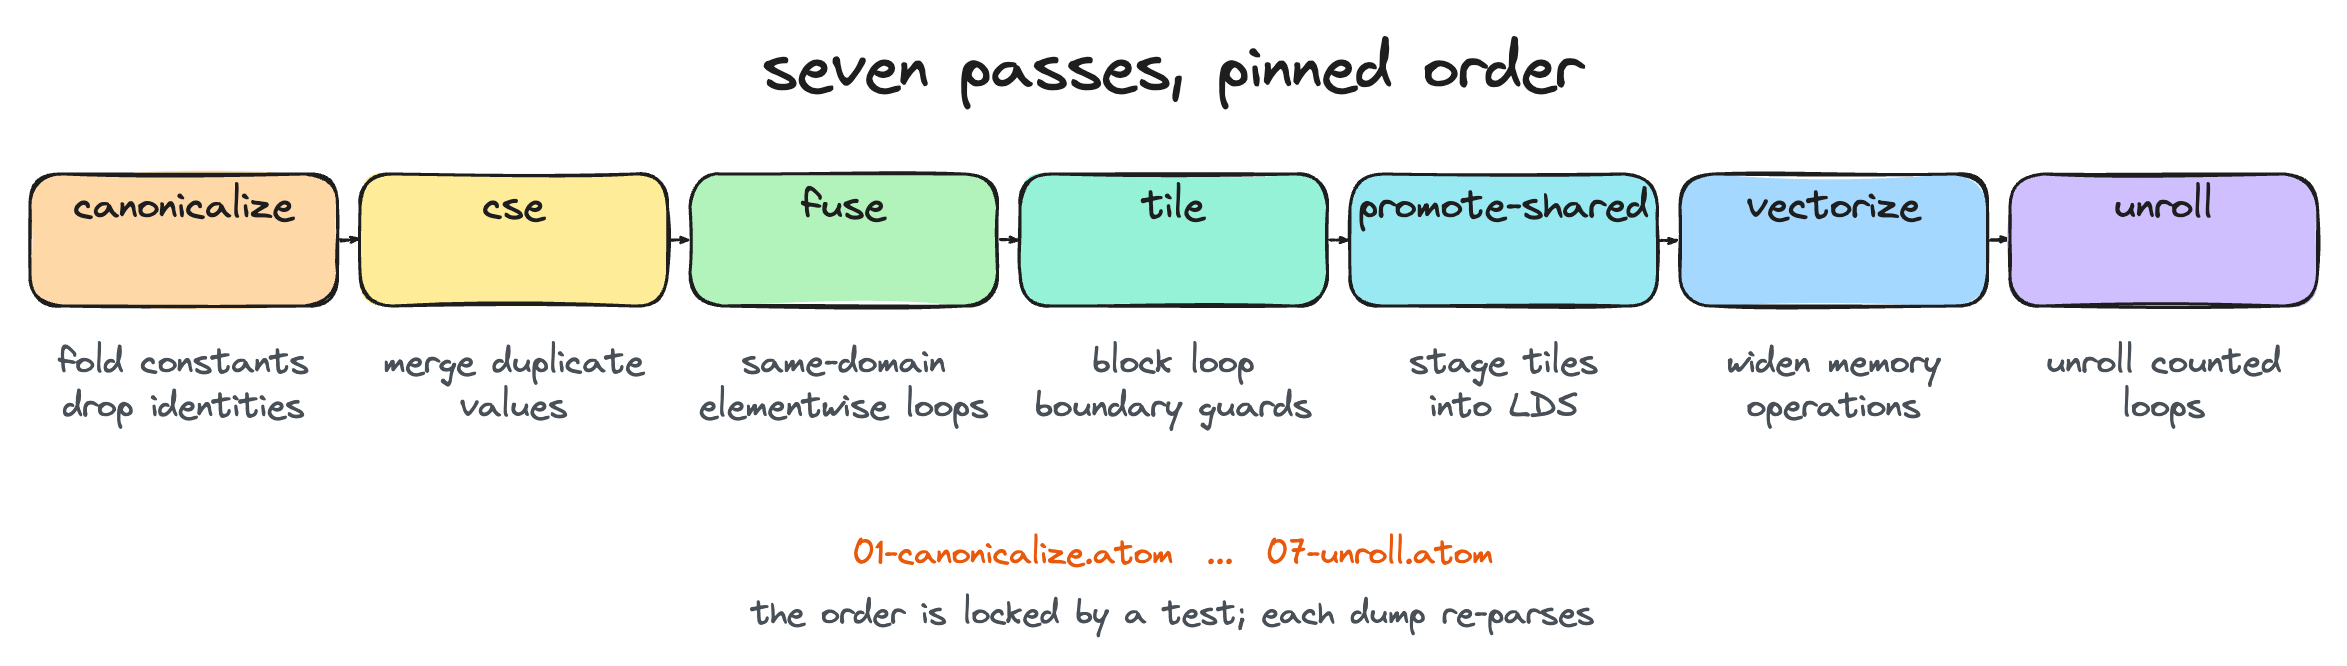
\includegraphics[width=\textwidth]{report-pipeline.png}
\caption{The seven-pass pipeline in canonical order
(\texttt{kernelh::passes::defaultPipelineOrder()}).}
\label{fig:passflow}
\end{figure}

\subsection{Before/After Excerpts}
\label{sec:pass-details}

\textbf{canonicalize (01).} GEMM's pre-pipeline input has no foldable constants: all
\texttt{atom.const} values are leaves. \texttt{01-canonicalize.atom} is byte-identical to
\texttt{00-input.atom}. The fusion example below shows a case where canonicalize did rewrite:
the \texttt{x + 0.0} identity elision is what lets the vectorizer widen the fused chain.

\textbf{cse (02).} \texttt{02-cse.atom} (3258\,B) is smaller than \texttt{00-input.atom}
(3461\,B). CSE merged duplicate constants (\texttt{\%v8 = atom.const 32} and
\texttt{\%v9 = atom.const 32}, which are different SSA ids with the same value, plus the
duplicate \texttt{1024} constants) and rewrote every use to the survivor.

\textbf{tile (04).} The domain loop \texttt{atom.loop\_for \%v3 to \%v4 step \%v7}
($0..256$ step 1) is rewritten into a block/tile loop. After the pass the kernel body starts
with \texttt{atom.block\_id x}, and the domain loop becomes:

\begin{lstlisting}[caption={Tiled domain loop (\texttt{04-tile.atom}).},label={lst:tile}]
  %v16 = atom.block_id x : index
  %v17 = atom.const 32 : index
  %v18 = atom.mul %v16, %v17 : index          ; base = block_id * 32
  ...
  atom.loop_for %v3 to %v28 step %v5 iter_args() -> () {
    ^bb0(%v29: index):
      %v30 = atom.mul %v29, %v25 : index
      %v31 = atom.add %v30, %v21 : index      ; row = i*W + wf
      %v32 = atom.add %v18, %v31 : index      ; gi = base + row
      %v33 = atom.cmp lt %v31, %v17 : index   ; ok_tile guard
      ...
\end{lstlisting}

The tile guard (\texttt{select(ok, gi, 0)}) wraps exactly the A-load and the C-store, the only
two uses of the induction \texttt{i}. GEMM's \texttt{04} is identical to
\texttt{05}/\texttt{06}/\texttt{07}: promote-shared is a no-op on the pre-staged template, and
\texttt{vector\_width=1} with \texttt{unroll=1} leaves the IR unchanged. The explore
self-check asserts this idempotency.

\textbf{Fusion before and after.} The fused\_gelu explore run
(\texttt{kernelh explore --kernel fused\_gelu --shape n=1048576 --target amdgcn-gfx1101})
produced the two dumps below. Before (\texttt{02-cse.atom}): two same-domain loops with an
intermediate \texttt{tensor<1048576xf32>} staging buffer. After (\texttt{03-fuse.atom}): one
loop computes the whole chain pointwise. The intermediate buffer is gone, along with the
producer store and consumer load.

\begin{lstlisting}[caption={Fusion before (\texttt{02-cse.atom}): two loops + staging buffer.},
                   label={lst:fuse-before}]
  atom.loop_for %v15 to %v3 step %v16 iter_args() -> () {
    ^bb0(%v17: index):
      %v18 = atom.load %v0[%v17] : tensor<1048576xf32, global>
      %v19 = atom.fma %v4, %v18, %v5 : f32
      atom.store %v19, %v1[%v17] : tensor<1048576xf32, global>
      atom.yield
  }
  atom.loop_for %v14 to %v3 step %v15 iter_args() -> () {
    ^bb0(%v16: index):
      %v17 = atom.load %v1[%v16] : tensor<1048576xf32, global>
      %v18 = atom.mul %v17, %v17 : f32
      %v19 = atom.mul %v18, %v17 : f32
      ... tanh ...
      atom.store %v27, %v2[%v16] : tensor<1048576xf32, global>
      atom.yield
  }
\end{lstlisting}

\begin{lstlisting}[caption={Fusion after (\texttt{03-fuse.atom}): one loop, buffer gone.},
                   label={lst:fuse-after}]
  atom.loop_for %v14 to %v3 step %v15 iter_args() -> () {
    ^bb0(%v16: index):
      %v17 = atom.load %v0[%v16] : tensor<1048576xf32, global>
      %v18 = atom.fma %v4, %v17, %v5 : f32
      %v19 = atom.mul %v18, %v18 : f32
      %v20 = atom.mul %v19, %v18 : f32
      %v21 = atom.mul %v8, %v20 : f32
      %v22 = atom.add %v18, %v21 : f32
      %v23 = atom.mul %v7, %v22 : f32
      %v24 = atom.math tanh %v23 : f32
      %v25 = atom.add %v24, %v6 : f32
      %v26 = atom.mul %v5, %v18 : f32
      %v27 = atom.mul %v26, %v25 : f32
      atom.store %v27, %v2[%v16] : tensor<1048576xf32, global>
      atom.yield
  }
\end{lstlisting}

Fusion fires only on same-domain producer and consumer pairs with no barrier between them.
The barrier-separated negative fixture (\texttt{test/fixtures/chain\_barrier.atom}) is left
unchanged. This applies the elementwise fusion used by FlashAttention-style kernels
\cite{flashattn2022,flashattn2} at the IR level. The tile pass follows the polyhedral tiling
approach used by Tiramisu \cite{tiramisu2019}, expressed in a small structured-SSA form.

\section{MLIR Lowering}
\label{sec:mlir}

The lowering chain, all in \texttt{lib/compiler/emitter.cpp} (two stages), is:

\begin{center}
\ttfamily
atom IR $\xrightarrow{\text{lowerToAtomDialect}}$ atom dialect (tblgen)\\
$\xrightarrow{\text{lowerAtomToGpu}}$ gpu.module \{ memref.global addrspace-3, gpu.func with dynamic
memref args, scf.for / vector / arith / math \}\\
$\xrightarrow{\text{fuse + canonicalize + cse cleanup}}$ emitGpuModule
\end{center}

\subsection{Device-Only Decision and Rationale}
\label{sec:device-only}

The emitter produces a \texttt{gpu.module} with \texttt{gpu.func} kernels. It does not emit
\texttt{gpu.launch}, outline host code, or use \texttt{gpu-to-llvm} host machinery. kernel.h's
runtime (\S\ref{sec:runtime}) launches the kernels at the device ABI, so host launching stays
in the runtime and the compiler does not depend on the MLIR ExecutionEngine. The device
module is what the vendor serializers consume (\texttt{gpu-module-to-binary}), and the
descriptor ABI (\S\ref{sec:descriptor}) supplies the launch arguments. The runtime links no
MLIR.

\cref{lst:gpumlir} is the MLIR output, verbatim from
\texttt{artifacts/run-report-nv/gpu.mlir}. The vecadd \texttt{gpu.module} has the same shape
on the AMD side.

\begin{lstlisting}[caption={Verbatim \texttt{gpu.module} for vecadd (\texttt{gpu.mlir}).},
                   label={lst:gpumlir}]
module {
  gpu.module @kernelh {
    gpu.func @vecadd(%arg0: memref<?xf32>, %arg1: memref<?xf32>, %arg2: memref<?xf32>) attributes {kernel} {
      %c1024 = arith.constant 1024 : index
      %block_id_x = gpu.block_id  x
      %block_dim_x = gpu.block_dim  x
      %grid_dim_x = gpu.grid_dim  x
      %thread_id_x = gpu.thread_id  x
      %0 = arith.muli %block_id_x, %block_dim_x : index
      %1 = arith.addi %0, %thread_id_x : index
      %2 = arith.muli %block_dim_x, %grid_dim_x : index
      scf.for %arg3 = %1 to %c1024 step %2 {
        %3 = memref.load %arg0[%arg3] : memref<?xf32>
        %4 = memref.load %arg1[%arg3] : memref<?xf32>
        %5 = arith.addf %3, %4 : f32
        memref.store %5, %arg2[%arg3] : memref<?xf32>
      }
      gpu.return
    }
  }
}
\end{lstlisting}

Static shared memory uses addrspace-3 globals. A per-thread \texttt{alloca} would break
cross-thread exchange, because NVPTX treats \texttt{alloca addrspace(3)} as per-thread. The
GEMM shared buffer from \texttt{artifacts/run-report-amd/rocdl.mlir}:

\begin{lstlisting}[caption={Static-LDS lowering in the ROCDL module (\texttt{rocdl.mlir}).},
                   label={lst:rocdl}]
  gpu.module @kernelh [#rocdl.target<chip = "gfx1101">] attributes {llvm.data_layout = ...} {
    llvm.mlir.global external @gemm_shared_0() {addr_space = 3 : i32} : !llvm.array<2048 x f32> {
      %0 = llvm.mlir.undef : !llvm.array<2048 x f32>
      llvm.return %0 : !llvm.array<2048 x f32>
    }
    llvm.func @gemm(%arg0: !llvm.ptr, %arg1: !llvm.ptr, %arg2: i64, ... ) attributes {gpu.kernel, rocdl.kernel} {
      ...
\end{lstlisting}

Key lowering facts:
\begin{itemize}
  \item Kernel arguments are \textbf{dynamic-shape memref descriptors}
        (\texttt{memref<?xf32>}, \texttt{memref<?x?xf32>}). The descriptor ABI expands a
        rank-$N$ buffer to $2N+3$ argument slots: allocated ptr, aligned ptr, offset i64, $N$
        sizes, $N$ strides (\S\ref{sec:descriptor}).
  \item Loop bounds for dynamic args come from \texttt{memref.dim} at runtime, not the static
        atom type.
  \item \texttt{atom.reduce} lowers to nested \texttt{scf.for} + iter\_args;
        \texttt{atom.copy} to nested \texttt{scf.for} + memref loads/stores.
  \item Custom cmp (i32 carrier) lowers to \texttt{arith.extui}, and select lowers to
        \texttt{arith.trunci}. Canonicalize folds \texttt{trunci(extui(cmp))} back to a
        plain \texttt{cmpf} plus \texttt{select}.
  \item The emitter's literal \texttt{kernel} marker attr is normalized to \texttt{gpu.kernel}
        inside the backend shim (\texttt{normalizeKernelMarkers}) so NVPTX/ROCDL emit
        \texttt{.visible .entry} / proper kernels.
\end{itemize}

\section{Vendor Backends}
\label{sec:backends}

Two vendor paths in \texttt{lib/compiler/backends.cpp}; each consumes a \emph{fresh clone} of
the \texttt{gpu.module} per artifact because \texttt{gpu-module-to-binary} mutates the module
in place. Both paths use LLVM's code-generation infrastructure \cite{llvm2004}, invoked
through the MLIR \texttt{gpu}-to-NVVM/ROCDL conversions (\S\ref{sec:mlir}).

\subsection{Verbatim PTX (NVIDIA, cross-compiled sm\_80)}
\label{sec:ptx}

\cref{lst:ptx} is verbatim from \texttt{artifacts/run-report-nv/vecadd.ptx} (the whole kernel
of the explore run \texttt{kernelh explore --kernel vecadd --shape n=1024 --target
nvptx-sm\_80}):

\begin{lstlisting}[caption={PTX for vecadd, sm\_80 (\texttt{vecadd.ptx}).},
                   label={lst:ptx}]
// Generated by LLVM NVPTX Back-End
//
.version 7.0
.target sm_80
.address_size 64

.visible .entry vecadd(
	.param .u64 .ptr .align 1 vecadd_param_0,
	.param .u64 .ptr .align 1 vecadd_param_1,
	.param .u64 vecadd_param_2,
	.param .u64 vecadd_param_3,
	.param .u64 vecadd_param_4,
	.param .u64 .ptr .align 1 vecadd_param_5,
	...
	.param .u64 vecadd_param_14
)
{
	.reg .pred 	%p<3>;
	.reg .b32 	%r<8>;
	.reg .b64 	%rd<22>;

	ld.param.b64 	%rd12, [vecadd_param_1];
	cvta.to.global.u64 	%rd1, %rd12;
	...
	mov.u32 	%r1, %ctaid.x;
	mov.u32 	%r2, %ntid.x;
	mov.u32 	%r4, %tid.x;
	cvt.u64.u32 	%rd15, %r4;
	mul.wide.u32 	%rd16, %r1, %r2;
	add.s64 	%rd20, %rd16, %rd15;
	setp.gt.u64 	%p1, %rd20, 1023;
	@%p1 bra 	$L__BB0_3;
	...
$L__BB0_2:
	add.s64 	%rd17, %rd1, %rd21;
	ld.global.b32 	%r5, [%rd17];
	add.s64 	%rd18, %rd2, %rd21;
	ld.global.b32 	%r6, [%rd18];
	add.rn.f32 	%r7, %r5, %r6;
	add.s64 	%rd19, %rd3, %rd21;
	st.global.b32 	[%rd19], %r7;
	add.s64 	%rd21, %rd21, %rd7;
	add.s64 	%rd20, %rd20, %rd5;
	setp.lt.u64 	%p2, %rd20, 1024;
	@%p2 bra 	$L__BB0_2;
$L__BB0_3:
	ret;
}
\end{lstlisting}

The \texttt{.visible .entry} directive, the \texttt{.target sm\_80} line, and the 15
descriptor parameters (3 memrefs $\times$ 5 slots) confirm the kernel-marker fix and the
descriptor ABI.

\subsection{Verbatim gfx1101 ISA (AMD, executed locally)}
\label{sec:isa}

\cref{lst:isa} is verbatim from \texttt{artifacts/run-report-amd/gemm.isa}: the header and
the k-accumulate loop with LDS traffic.

\begin{lstlisting}[caption={gfx1101 ISA for the tiled GEMM (\texttt{gemm.isa}).},
                   label={lst:isa}]
	.amdgcn_target "amdgcn-amd-amdhsa--gfx1101"
	.amdhsa_code_object_version 6
	.text
	.globl	gemm
	.p2align	8
	.type	gemm,@function
gemm:
	s_load_b32 s3, s[0:1], 0xb4
	v_and_b32_e32 v7, 31, v0
	v_dual_mov_b32 v1, 0 :: v_dual_and_b32 v6, 0xe0, v0
	s_clause 0x5
	s_load_b64 s[10:11], s[0:1], 0x78
	...
	v_cvt_f32_u32_e32 v2, s17
	...
	v_mul_f32_e32 v7, v19, v5
	...
\end{lstlisting}

...and the compute loop. The \texttt{ds\_} loads show the LDS path; \texttt{v\_fmac\_f32} is
the accumulator FMA, with 32 occurrences in this ISA:

\begin{lstlisting}[caption={gfx1101 k-accumulate loop with LDS traffic (\texttt{gemm.isa}).},
                   label={lst:isaloop}]
	ds_store_b32 v29, v30
	...
	s_waitcnt lgkmcnt(0)
	s_waitcnt_vscnt null, 0x0
	s_barrier
	buffer_gl0_inv
	ds_load_b128 v[29:32], v12
	ds_load_2addr_b32 v[6:7], v16 offset1:32
	ds_load_2addr_b32 v[37:38], v16 offset0:64 offset1:96
	ds_load_b128 v[33:36], v12 offset:16
	ds_load_2addr_b32 v[39:40], v16 offset0:128 offset1:160
	...
	v_fmac_f32_e32 v28, v29, v6
	s_delay_alu instid0(VALU_DEP_1) | instskip(SKIP_3) | instid1(VALU_DEP_1)
	v_fmac_f32_e32 v28, v30, v7
	...
\end{lstlisting}

ISA-wide totals (\texttt{grep -c} on the artifact): \texttt{ds\_load}/\texttt{ds\_store}/
\texttt{s\_barrier} 30 matches, \texttt{v\_fmac\_f32} 32. The embedded amdhsa metadata tail
pins the resource usage: \texttt{.group\_segment\_fixed\_size: 8192},
\texttt{.vgpr\_count: 41}, \texttt{.sgpr\_count: 26}, \texttt{.wavefront\_size: 32},
\texttt{.max\_flat\_workgroup\_size: 256}, and \texttt{.kernarg\_segment\_size: 424}. These
values match \texttt{resources.json} (vgpr 41, sgpr 26, lds 8192).

\subsection{Serialization Mechanics}
\label{sec:serialization}

\texttt{gpu-module-to-binary} runs vendor linkers and does not touch a GPU:
\begin{itemize}
  \item \textbf{ROCDL \texttt{format=bin}} (HSACO): requires the ROCm toolkit:
        \texttt{<toolkit>/llvm/bin/ld.lld} (an \emph{external} linker, LLD 22.0.0
        rocm-7.2.3) plus the device-libs at \texttt{<toolkit>/amdgcn/bitcode/}
        (\texttt{ocml.bc}, \texttt{ockl.bc}, \texttt{hip.bc}, \texttt{opencl.bc} + 67
        \texttt{oclc\_*} control bitcodes; 71 files total). The \texttt{rocm-toolkit-root}
        linkFarm aggregate remaps
        \texttt{\$\{rocmPackages.llvm.lld\}/bin/ld.lld $\to$ llvm/bin/ld.lld} and every
        \texttt{\$\{rocmPackages.rocm-device-libs\}/amdgcn/bitcode/*.bc $\to$ amdgcn/bitcode/}.
        Toolkit is wired via \texttt{ROCM\_TOOLKIT\_ROOT}; a bogus toolkit path fails cleanly
        with the serializer's own error, and \texttt{format=isa} still requires the toolkit
        because the serializer drives the same ld.lld path.
  \item \textbf{NVVM \texttt{format=bin}} (cubin): needs \texttt{ptxas} (CUDA 12.9,
        \texttt{Build cuda\_12.9.r12.9/compiler.36037853\_0}) and libdevice
        (\texttt{nvvm/libdevice/libdevice.10.bc}, passed through the pass's own \texttt{l=}
        linkFiles option, separate from \texttt{opts=}), both from the
        \texttt{cuda-toolkit-root} aggregate. \texttt{format=isa} (PTX text) needs no toolkit.
  \item Valid format strings are \texttt{offloading|llvm|assembly|isa|binary|bin|
        fatbinary|fatbin}. The codebase does not use ``asm''.
  \item \textbf{Blob extraction}: after \texttt{gpu-module-to-binary} the module holds
        \texttt{gpu.binary [\#gpu.object<target, bin = "...">]}; \texttt{compileToBlob} walks
        for the \texttt{BinaryOp}, matches the object's \texttt{CompilationTarget}, and reads
        the raw payload StringAttr (in memory it is raw bytes; MLIR escaping happens at print
        time). Verified artifacts start with the ELF magic \texttt{7f 45 4c 46}; the cubin
        \texttt{llvm-readobj -h} reports \texttt{Machine: EM\_CUDA (0xBE)}.
\end{itemize}

Artifact sizes: \texttt{gemm.hsaco} 6528\,B (ELF, 3 amdhsa note sections),
\texttt{gemm.isa} 14\,877\,B, \texttt{vecadd.cubin} 3496\,B (EM\_CUDA),
\texttt{vecadd.ptx} 1619\,B.

\section{Runtime and Loading}
\label{sec:runtime}

The runtime is plain C++ (\texttt{lib/runtime}, linked with clang and
\texttt{-lamdhip64}, with HIP type-free headers; it does not use hipcc). The local path:

\begin{itemize}
  \item \texttt{DeviceContext::create} $\to$ \texttt{hipSetDevice(0)} + live queries
        (device name ``AMD Radeon RX 7800 XT'', 30 CUs, 64\,KiB LDS, wavefront 32, max threads
        1024; all agree with the gfx1101 device-limits table entry).
  \item \texttt{GpuModule::load(image, size)} $\to$ \textbf{\texttt{hipModuleLoadData}}
        $\to$ \texttt{get\_function} $\to$ \textbf{\texttt{hipModuleGetFunction}} $\to$
        \texttt{KernelLaunch.launch(fn)} $\to$ \textbf{\texttt{hipModuleLaunchKernel}}. The
        launch uses \texttt{sharedMemBytes=0} (the v1 ABI uses static LDS only) and
        descriptor-packed \texttt{kernelParams}.
\end{itemize}

\subsection{Descriptor ABI}
\label{sec:descriptor}

Each rank-$N$ buffer uses five slots for 1-D and eleven for rank-2: allocated pointer,
aligned pointer, offset i64(0), $N$ sizes, and $N$ strides. Strides are emitted
dim-0-first ($16\times 8 \to$ strides \texttt{[8,1]}). Scalars follow by value.
\texttt{LaunchArgs::params()} returns the \texttt{void**} array pointing at each slot.
This matches the MLIR memref descriptor layout used by the vendor lowering
(\S\ref{sec:mlir}).

\subsection{CUDA Backend (cross-ready, not linked)}
\label{sec:cuda}

The same interface is implemented over the CUDA Driver API bound at runtime via
\texttt{dlopen("libcuda.so.1")} + \texttt{dlsym} of 24 symbols (\texttt{cuInit},
\texttt{cuDeviceGet}, \texttt{cuModuleLoadData}, \texttt{cuModuleGetFunction},
\texttt{cuLaunchKernel}, \texttt{cuEvent*}, \texttt{cuMemAlloc\_v2}/\texttt{cuMemFree\_v2}/
\texttt{cuMemcpyHtoD\_v2}/\texttt{cuMemcpyDtoH\_v2}, \dots). If \texttt{dlopen} fails every
call returns a clean error (\texttt{kCudaDriverUnavailable}), and \texttt{kernelh bench} on
NVIDIA targets exits 77 (skip). \texttt{ldd} on the binary shows zero \texttt{libcuda}
references.

\textbf{Three CUDA backend bugs.} The first run on an RTX 6000 Ada pod exposed three bugs
that the local dlopen-failure path had hidden:
\begin{enumerate}
  \item \textbf{dlsym names}: the table asked for CamelCase names (\texttt{CuInit},
        \texttt{CuDeviceGet}, \dots), but the driver exports lowercase names (\texttt{cuInit},
        \texttt{cuDeviceGet}, \dots). The live GPU returned ``\texttt{dlsym(CuInit) failed}''.
  \item \textbf{\_v2 variants}: \texttt{cuMemAlloc}/\texttt{cuMemFree}/
        \texttt{cuMemcpyHtoD}/\texttt{cuMemcpyDtoH} (deprecated aliases) return
        \texttt{CUDA\_ERROR\_INVALID\_CONTEXT} (201) even with the primary context current on
        that driver; \texttt{cuMemAlloc\_v2}/\texttt{cuMemFree\_v2}/\texttt{cuMemcpyHtoD\_v2}/
        \texttt{cuMemcpyDtoH\_v2} succeed. Fixed to the \texttt{\_v2} variants (verified
        present via \texttt{nm -D}).
  \item \textbf{Attribute IDs}: the warp size used 39 (=
        \texttt{CU\_DEVICE\_ATTRIBUTE\_MAX\_THREADS\_PER\_MULTIPROCESSOR}, returned 1536)
        instead of 10 (returned 32); \texttt{MultiProcessorCount} used 41 instead of 16
        (returned 1; RTX 6000 Ada has 142 SMs). Fixed per \texttt{cuda.h} CUDA 12.9.
\end{enumerate}

The full path (DSL, pipeline, emitter, NVVM cubin, descriptor-ABI launch, numeric
verification) runs on NVIDIA hardware (\S\ref{sec:validation}).

\section{Autotuning}
\label{sec:autotune}

\texttt{kernelh tune} (\texttt{lib/compiler/autotuner.cpp} + the CLI driver in
\texttt{tools/kernelh/main.cpp}) is GEMM-only in v1.

\textbf{Config space} (\texttt{gemm\_config\_space()}): 216 = $3\text{(bm)} \times
3\text{(bn)} \times 2\text{(bk)} \times 2\text{(waves)} \times 2\text{(unroll)} \times
3\text{(vec)}$, with bm/bn $\in$ \{64,128,256\}, bk $\in$ \{16,32\}, waves $\in$ \{4,8\},
unroll $\in$ \{1,2\}, vec $\in$ \{1,2,4\}. \texttt{--max-candidates} caps the number
evaluated; \texttt{--sample} sizes the fixed-seed random sample; \texttt{--refine-budget}
bounds best-neighbor refinement.

\textbf{Evaluation gates}, in order, in a forked child with a wall-clock deadline:
\begin{enumerate}
  \item Compile for the tuning shape; an LDS/shared-memory compile error is surfaced as
        \texttt{pruned: lds}.
  \item Launch verification $\to$ \texttt{pruned: launch}.
  \item Resource check (\texttt{resources.json} on the actual artifact) $\to$
        \texttt{pruned: vgpr} / \texttt{pruned: lds} if the kernel cannot be resident
        (the profiler-feedback seam).
  \item \textbf{Mandatory numeric re-verification} on a small shape ($\le 128$/dim) against
        the fp64 reference, tolerance rel-Frobenius $\le 1e-5$. Any candidate that fails is
        discarded. The gate accepts a candidate only after numeric re-verification.
  \item EventTimer timing (warmup 3, median 10) on the tuning shape for accepted candidates.
\end{enumerate}

\textbf{Cache:} whole-run JSON cache (\texttt{build/tune-cache.json}, hand-rolled JSON
writer) keyed \texttt{sha256(kernel+shape+device\_name)}. A second run with the same key is
served entirely from cache.

\textbf{Recorded run.} \texttt{tune-results.csv} holds the verbatim results for 8
candidates at \texttt{m=512,n=512,k=512} with \texttt{--max-candidates 8}:

\begin{lstlisting}[caption={Autotune results: a negative result
(\texttt{tune-results.csv}).},label={lst:tune},basicstyle=\ttfamily\scriptsize,
                   breaklines=true,breakatwhitespace=false,
                   postbreak=\mbox{\textcolor{red}{$\hookrightarrow$}\space}]
kernel,shape,bm,bn,bk,waves,unroll,vec,ms_median,accepted,reason
gemm,"k=512,m=512,n=512",64,64,16,4,1,2,0,false,reverify: FAIL (rel-frobenius 0.7071607398 > 1e-5)
gemm,"k=512,m=512,n=512",128,128,16,8,1,1,0,false,reverify: FAIL (rel-frobenius 0.8660254038 > 1e-5)
gemm,"k=512,m=512,n=512",128,64,32,8,2,4,0,false,reverify: FAIL (rel-frobenius 0.8837545775 > 1e-5)
gemm,"k=512,m=512,n=512",256,64,32,8,1,2,0,false,reverify: FAIL (rel-frobenius 0.7072175998 > 1e-5)
gemm,"k=512,m=512,n=512",128,256,16,8,2,1,0,false,reverify: FAIL (rel-frobenius 0.9703290074 > 1e-5)
gemm,"k=512,m=512,n=512",256,128,32,8,1,2,0,false,reverify: FAIL (rel-frobenius 0.8660397367 > 1e-5)
gemm,"k=512,m=512,n=512",64,256,32,4,1,4,0,false,reverify: FAIL (rel-frobenius 0.8660456794 > 1e-5)
gemm,"k=512,m=512,n=512",128,64,32,4,2,4,0,false,reverify: FAIL (rel-frobenius 0.8835009408 > 1e-5)
\end{lstlisting}

All eight candidates failed numeric re-verification. The three unroll=2 candidates
(0-based indices 2, 4, and 7; rel-Frobenius 0.883--0.970) trace to the unroll pass: its
partial-unroll cleanup loop mis-remaps the k-loop iter\_args carry chain and corrupts the
accumulator. The five unroll=1 candidates failed the same gate; this report does not diagnose
those failures. The gate rejected every candidate, and the search ended with \texttt{no
accepted candidate} and \texttt{skipping refinement}, so no broken configuration shipped. The run logs
\texttt{cache-miss} on the first pass, \texttt{cache-hit} and \texttt{tune ok (served from
cache)} on the rerun, and \texttt{best config: none (no candidate passed all gates)}.

\section{Performance}
\label{sec:perf}

All numbers below are measurements from \path{build/bench/results.csv}, generated by
\texttt{kernelh bench --suite all --out build/bench} with warmup 5 and the median of 20
GPU-event-timed launches on an AMD Radeon RX 7800 XT.

\subsection{Measured Roofline Ceilings (this box)}
\label{sec:roofline}

\begin{table}[H]
\centering
\caption{Measured microbenchmark ceilings (\texttt{build/bench/results.csv}).}
\label{tab:roofline}
\begin{tabular}{@{}llrrc@{}}
\toprule
microbenchmark & shape & median \ms & rate \\
\midrule
\texttt{roofline\_triad} & $n=2^{28}$ per buffer (1 GiB $\times$ 3) & 9.26 & 347.8\gbs \\
\texttt{roofline\_fma} & $2^{22} \times 8192$ FMAs/thread & 4.42 & 15\,559.8\gflops \\
\bottomrule
\end{tabular}
\end{table}

The ridge point (arithmetic intensity where the two ceilings meet) is
$\mathrm{AI} = 15\,559.8\gflops / 347.8\gbs = 44.7$ flops/byte; the
\texttt{charts\_stats.csv} row carries the exact computed value \texttt{ceiling\_ai =
44.737538} with \texttt{ceiling\_gflops = 15559.795120}. \cref{fig:roofline} shows the
measured roofline \cite{roofline2009}, with the measured ceilings and the kernelh GEMM and
attention points plotted at their arithmetic intensities.

\begin{figure}[H]
\centering
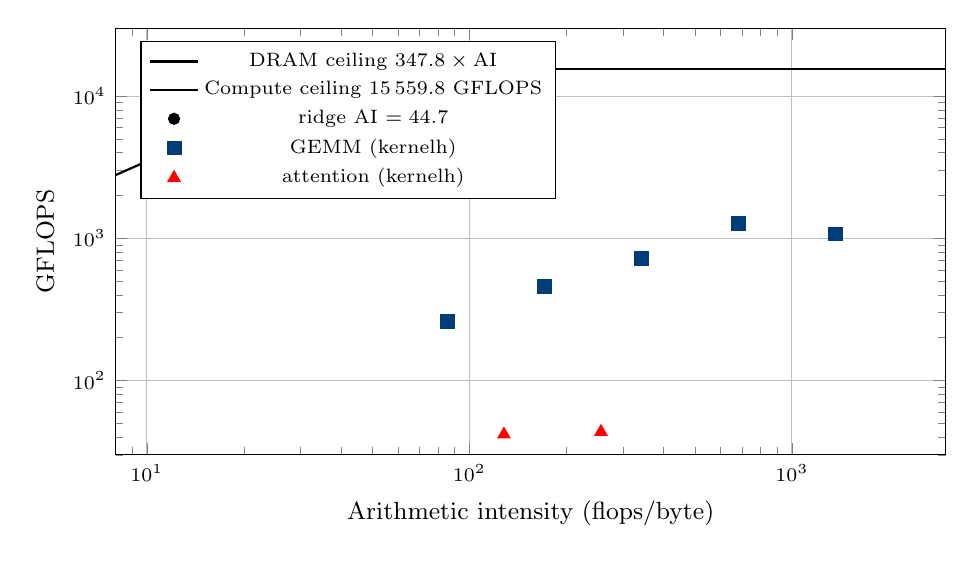
\begin{tikzpicture}
\begin{axis}[
  width=\textwidth, height=7cm,
  xmode=log, ymode=log,
  xlabel={Arithmetic intensity (flops/byte)},
  ylabel={GFLOPS},
  xmin=8, xmax=3000, ymin=30, ymax=30000,
  grid=major,
  legend pos=north west,
  legend style={font=\scriptsize},
  tick label style={font=\scriptsize},
  label style={font=\small},
]
  % DRAM ceiling: y = 347.8 * x  (up to ridge at AI=44.7)
  \addplot[domain=8:44.737538, samples=2, thick, black, solid]
    {347.8017752*x};
  \addlegendentry{DRAM ceiling $347.8\times\mathrm{AI}$}
  % Compute ceiling
  \addplot[domain=44.737538:3000, samples=2, thick, black, solid]
    {15559.795120};
  \addlegendentry{Compute ceiling $15\,559.8$ GFLOPS}
  % ridge marker
  \addplot[only marks, mark=*, mark size=2pt, black]
    coordinates {(44.737538, 15559.795120)};
  \addlegendentry{ridge AI $= 44.7$}
  % GEMM kernelh points (AI = N/6 for square)
  \addplot[only marks, mark=square*, mark size=2.5pt, accent]
    coordinates {(85.333333, 261.117763) (170.666667, 456.330662)
                 (341.333333, 718.384408) (682.666667, 1275.529751)
                 (1365.333333, 1072.524390)};
  \addlegendentry{GEMM (kernelh)}
  % attention points (AI = s/4)
  \addplot[only marks, mark=triangle*, mark size=2.5pt, red]
    coordinates {(128.000000, 41.781830) (256.000000, 43.574118)};
  \addlegendentry{attention (kernelh)}
\end{axis}
\end{tikzpicture}
\caption{Measured roofline \cite{roofline2009} for the RX 7800 XT: DRAM ceiling
(347.8\,GB/s $\times$ AI), FMA compute ceiling (15\,559.8\,GFLOPS), and the kernelh
GEMM/attention points from \texttt{charts\_stats.csv}. GEMM AI $= N/6$ (square), attention
AI $= s/4$.}
\label{fig:roofline}
\end{figure}

\subsection{GEMM: kernelh vs.\ rocBLAS}
\label{sec:gemm}

\begin{table}[H]
\centering
\caption{GEMM, kernelh vs.\ rocBLAS (numbers from \texttt{build/bench/results.csv}).}
\label{tab:gemm}
\begin{tabular}{@{}lrrrrr@{}}
\toprule
shape ($m{=}n{=}k$) & kernelh \ms & kernelh GFLOPS & rocBLAS \ms & rocBLAS GFLOPS & ratio \\
\midrule
$512^3$    & 1.028  & 261.1  & 0.0576 & 4658.7  & 17.8$\times$ \\
$1024^3$   & 4.706  & 456.3  & 0.281  & 7646.6  & 16.8$\times$ \\
$2048^3$   & 23.91  & 718.4  & 1.925  & 8925.3  & 12.4$\times$ \\
$4096^3$   & 107.75 & 1275.5 & 13.79  & 9970.2  & 7.8$\times$ \\
$8192^3$   & 1025.16& 1072.5 & 107.83 & 10\,196.5 & 9.5$\times$ \\
\bottomrule
\end{tabular}
\end{table}

\cref{fig:gemm} plots the same data (log-scale GFLOPS). The hipref-naive GEMM reference:
$512^3 \to$ 4497.9 GFLOPS, $1024^3 \to$ 6665.9.

\begin{figure}[H]
\centering
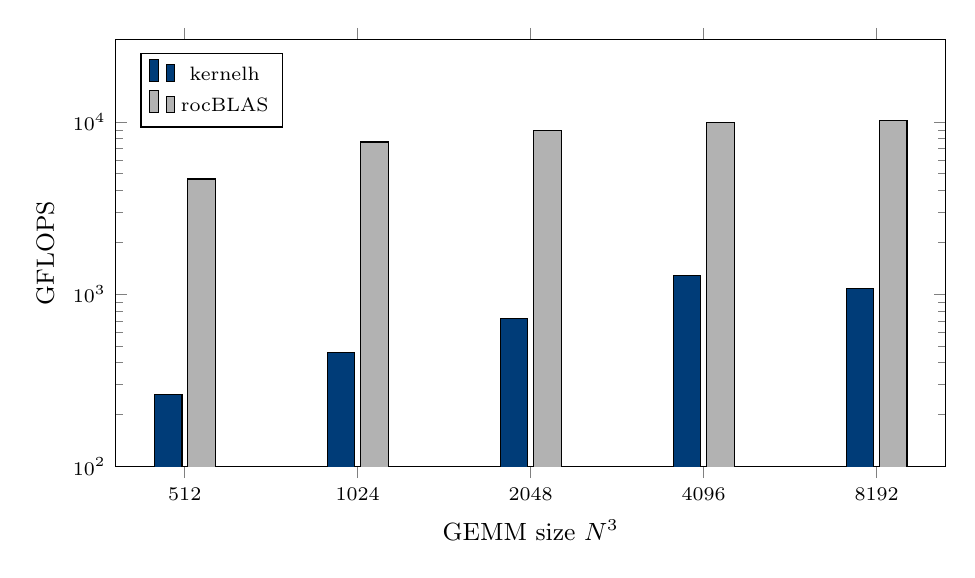
\begin{tikzpicture}
\begin{axis}[
  width=\textwidth, height=7cm,
  ybar, ymode=log, ymin=100, ymax=30000,
  bar width=10pt,
  symbolic x coords={512,1024,2048,4096,8192},
  xtick=data,
  xlabel={GEMM size $N^3$},
  ylabel={GFLOPS},
  legend pos=north west,
  legend style={font=\scriptsize},
  tick label style={font=\scriptsize},
  label style={font=\small},
  nodes near coords={},
]
  \addplot[fill=accent] coordinates {(512,261.1) (1024,456.3) (2048,718.4) (4096,1275.5) (8192,1072.5)};
  \addlegendentry{kernelh}
  \addplot[fill=gray!60] coordinates {(512,4658.7) (1024,7646.6) (2048,8925.3) (4096,9970.2) (8192,10196.5)};
  \addlegendentry{rocBLAS}
\end{axis}
\end{tikzpicture}
\caption{GEMM GFLOPS vs.\ size: kernelh (scalar, tiled, static shared memory) vs.\ rocBLAS
(same box, same fp32). Data from \texttt{build/bench/results.csv}.}
\label{fig:gemm}
\end{figure}

\textbf{The GEMM gap.} kernel.h's GEMM is a scalar, tiled, static-shared-memory kernel that
uses f32 FMA; tensor cores and WMMA are out of scope (\S\ref{sec:limitations}). At
$8192^3$ it is about 9.5$\times$ slower than rocBLAS (1072.5 vs.\ 10\,196.5 GFLOPS). The gap
is largest at small sizes (17.8$\times$ at $512^3$), where rocBLAS's tuned inner kernel and
launch overhead dominate. The relative gap narrows as $N$ grows: tile efficiency improves,
although the $8192^3$ kernelh run is the slowest cell in the suite at 1025\,ms. The best
kernelh cell (1275.5 GFLOPS at $4096^3$) reaches about 8\% of the measured FMA ceiling
(15\,559.8 GFLOPS). The causes are scalar accumulation with a $32\times32\times32$ tile,
12.5\% occupancy (\S\ref{sec:occupancy}), no double-buffered pipeline, and about 30\% of peak
LDS bandwidth used by the \texttt{ds\_load\_2addr} pattern. rocBLAS also avoids WMMA on
gfx1101; it uses register-blocked accumulation, wider tiles, and aggressive pipelining. Those
are v1 scope-outs. The design space is covered by CUTLASS \cite{cutlass_github}, cuBLAS
\cite{cublas_docs}, and rocBLAS \cite{rocblas_docs}.

\subsection{Elementwise / Reduction Kernels}
\label{sec:elem}

\begin{table}[H]
\centering
\caption{Elementwise / reduction kernels (numbers from \texttt{build/bench/results.csv}).}
\label{tab:elem}
\begin{tabular}{@{}llrrr@{}}
\toprule
kernel & shape & kernelh & hipref-naive & hipref-vec \\
\midrule
softmax    & $4096\times1024$  & 8.5\gbs   & 475.5\gbs & 717.0\gbs \\
softmax    & $16384\times4096$ & 9.6\gbs   & 424.2\gbs & 492.4\gbs \\
layernorm  & $4096\times1024$  & 69.0\gbs  & 472.7\gbs & 709.0\gbs \\
layernorm  & $16384\times4096$ & 68.3\gbs  & 410.2\gbs & 489.1\gbs \\
scan       & 100\,000          & 3.16\gbs  & 3.68\gbs  & 3.69\gbs \\
scan       & 1\,000\,000        & 3.57\gbs  & 4.35\gbs  & 4.27\gbs \\
fused\_gelu & $2^{20}$         & 627.9\gbs & 663.7\gbs & 706.9\gbs \\
fused\_gelu & $2^{22}$         & 1110.1\gbs & 1160.8\gbs & 1072.3\gbs \\
attention & $b{=}2,h{=}8,\mathrm{seq}{=}512$  & 41.8\gflops & n/a & n/a \\
attention & $b{=}2,h{=}8,\mathrm{seq}{=}1024$ & 43.6\gflops & n/a & n/a \\
\bottomrule
\end{tabular}
\end{table}

\textbf{Analysis.}
\begin{itemize}
  \item \textbf{fused\_gelu} is close to the HIP references and faster at $2^{22}$. The fusion
        pass (\S\ref{sec:pass-details}) removes the intermediate tensor's global round-trip.
        Its 1100\,GB/s exceeds the 347.8\,GB/s triad ceiling because the triad microbenchmark
        streams 3\,GiB (DRAM-bound) while fused\_gelu's 16\,MiB working set stays in L1/L2.
        The triad ceiling is a DRAM ceiling; small working sets can sit above it.
  \item \textbf{softmax and layernorm are the weak spot}: 8.5--69\,GB/s against 400--700\,GB/s
        for the HIP references, a 10--80$\times$ gap. These kernels are bandwidth-bound. The
        HIP references use float4 vectorization; the kernelh templates run scalar
        (\texttt{vector\_width=1} in the default schedule). The measured rates show a v1
        codegen inefficiency.
  \item \textbf{scan} is near parity (3.16--3.57 vs.\ 3.68--4.35\,GB/s). The two-pass
        Blelloch cost shows up as the flat low rate; both implementations are bandwidth-bound.
  \item \textbf{attention} has no local vendor baseline. rocBLAS lacks an attention API, and
        the cuBLAS/CUTLASS rows skip with exit 77 because this box has no NVIDIA driver. The online,
        tiled, fp32 attention reaches about 43.6\,GFLOPS at seq=1024 (AI $= s/4 = 256$
        flops/byte, in the compute region of the roofline). The achieved point sits below the
        FMA ceiling, as expected for a small, low-occupancy kernel at 3.125\% occupancy
        (\S\ref{sec:occupancy}). It is a FlashAttention-lite \cite{flashattn2022,flashattn2}
        realization with online rescaling, per-tile LDS staging, and fp32.
\end{itemize}

\subsection{Occupancy}
\label{sec:occupancy}

From \texttt{build/bench/occ/occupancy.md}. Theoretical occupancy comes from the resource
reports and the device-limits table. Measured occupancy is ``n/a'' on this box:
\texttt{hipOccupancyMaxActive\-Blocks\-Per\-Multiprocessor} returns
\texttt{hipErrorInvalidDeviceFunction} for every kernel under ROCm 7.2.3 and this kernel. The
analytic fallback is the only working path.

\begin{table}[H]
\centering
\caption{Occupancy table (theoretical; measured n/a on this driver stack).}
\label{tab:occ}
\begin{tabular}{@{}llrrrrl@{}}
\toprule
kernel & config & vgpr & lds (B) & theoretical \% & measured \% & limiter \\
\midrule
gemm & $512^3\dots 8192^3$ & 41 & 8192 & 12.5 & n/a & vgpr \\
softmax & $4096\times1024$ / $16384\times4096$ & 48 & 0 & 12.5 & n/a & vgpr \\
layernorm & $4096\times1024$ / $16384\times4096$ & 12 & 0 & 12.5 & n/a & threads \\
scan & $10^5$ / $10^6$ & 21 & 3072 & 12.5 & n/a & threads \\
fused\_gelu & $2^{20}$ / $2^{22}$ & 10 & 0 & 12.5 & n/a & threads \\
attention & seq=512/1024 & 27 & 33\,024 & 3.125 & n/a & lds \\
\bottomrule
\end{tabular}
\end{table}

\textbf{Analysis.} 12.5\% theoretical occupancy is low. The GEMM limiter is VGPRs (41
VGPRs/kernel, so $\lfloor 6144/(41\times32)\rfloor = 4$ waves of 32 per CU against 32
waves/CU). The attention kernel is LDS-limited at 3.125\%: its K/V/Q staging footprint is
33\,024\,B of the 65\,536\,B budget, which admits one block per CU. The v1 static-LDS
design sets these ceilings. Register blocking and shared-memory double buffering are future
work (\S\ref{sec:limitations}). The measured-to-theoretical gap comes from the platform.

\section{Validation and Failure Evidence}
\label{sec:validation}

\textbf{This box runs in full runtime mode.} \texttt{.omo/evidence/degraded.flag} contains
\texttt{degraded=false} (15 bytes, written by the AMD runtime smoke gate). All
\texttt{[gpu]}-tagged e2e tests execute on the GPU; none skip.

\begin{itemize}
  \item \textbf{AMD runtime gate}: \texttt{rocminfo} shows Agent gfx1101 (AMD Radeon RX
        7800 XT) with \texttt{KERNEL\_DISPATCH}; \texttt{HSA\_OVERRIDE\_GFX\_VERSION} is unset;
        the hipcc vectorAdd binary prints \texttt{VECTORADD-PASS} 2/2 ($2^{20}$ elements,
        host-side exact compare); a HIP module-loader probe compiles.
  \item \textbf{MLIR ROCDL pipeline gate}: a hand-authored \texttt{gpu.module} with a
        cross-thread LDS exchange lowered to gfx1101 HSACO (10\,208\,B, ELF magic, 3 amdhsa
        note sections, \texttt{group\_segment\_fixed\_size: 1024}, 8 \texttt{ds\_}
        instructions, \texttt{s\_barrier}), loaded via the production module loader and
        executed: \texttt{LOAD-MODULE-PASS} 2/2 with full-array host-side numeric
        verification. A bogus toolkit path fails cleanly naming the ROCm path.
  \item \textbf{Kernel e2e on the live GPU} (Catch2 \texttt{[gpu]}): vecadd
        \texttt{max-abs-diff=0.000000000} at 1024/65\,536/$2^{20}$; softmax worst
        \texttt{max-abs-diff=0.000000004}; GEMM \texttt{rel-frobenius=0.000000e+00} at all 6
        sizes including the $1000^3$ boundary; attention \texttt{max-abs-diff}
        $\sim 1.5e{-}7$; the \texttt{[!shouldfail]} negative controls all fire; the canary
        prints \texttt{CANARY-GPU-PASSED}. Full suite: 324/324 ctest tests pass (unit + lit
        + on-GPU e2e).
  \item \textbf{Runtime e2e}: the MLIR-emitted \texttt{xchg.hsaco} runs through the
        descriptor-ABI runtime (\texttt{RUNTIME-XCHG-PASS}, $N=1<<20$).
  \item \textbf{NVIDIA live validation} (RTX 6000 Ada pod, PrimeIntellect): the full path from
        DSL through pipeline, emitter, and NVVM cubin to the descriptor-ABI launch and numeric
        verification runs on NVIDIA hardware: \texttt{NV-BACKEND-OK}, \texttt{NV-DEVICE}
        (cu=142 lds=49\,152 wavefront=32 maxThreads=1024), \texttt{NV-MODULE-LOAD-OK},
        \texttt{NV-LAUNCH-OK} (grid=4096 block=256), \texttt{NV-VECADD-PASS} ($N{=}2^{20}$,
        host-side verified). Driver 580.126.09 (CUDA 13.0).
  \item \textbf{Bench and runtime failures exit with a message}: clock pinning emits EPERM
        warnings and falls back to median-of-20; a missing CUDA driver exits 77 with a
        message; a hung autotune candidate is SIGKILLed and recorded \texttt{timeout}; broken
        per-pass dumps make \texttt{kernelh explore} exit 1 and name the file.
\end{itemize}

One failure did occur. The original serial GEMM caused a GPU hang that killed the desktop
session at $8192^3$: about 44\,s per launch, 25 launches, which exceeded the AMD
lockup\_timeout. Root cause: the nested global loads could not be staged by promote-shared, so
the HSACO had \texttt{group\_segment\_fixed\_size: 0} and no \texttt{ds\_} instructions, and
all 256 threads redundantly computed the whole product at about 12 GFLOPS. The fix rewrites
the template to pre-stage tiles through static LDS. The fixed kernel runs $8192^3$ in
1005--1025\,ms with \texttt{group\_segment\_fixed\_size: 8192} and 18--30 \texttt{ds\_}
instructions.

\section{Limitations}
\label{sec:limitations}

\begin{enumerate}
  \item \textbf{Tensor cores are out of scope.} gfx1101 WMMA is untrusted upstream
        (ROCm/ROCm\#6349 \cite{rocm_github}); the plan greps kernels/lib for
        \texttt{wmma}/\texttt{mfma} and requires zero hits. GEMM and attention use scalar f32
        FMAs, which caps them below the vendor libraries (\S\ref{sec:gemm}).
  \item \textbf{NVIDIA code is cross-compiled here.} No NVIDIA hardware is local. Every
        NVIDIA artifact is emitted and the blobs are verified (ELF/PTX magic,
        \texttt{.target sm\_80}, \texttt{Machine: EM\_CUDA}), then exercised on a rented
        RTX 6000 Ada pod, where the full path runs and numerically verifies
        (\texttt{NV-VECADD-PASS}). \texttt{kernelh bench} NVIDIA rows exit 77 locally because
        no CUDA driver is present.
  \item \textbf{Unofficial distro and kernel.} The host is a rolling distro with an in-tree
        AMD driver and kernel. It is smoke-gated and works (\S\ref{sec:validation}), but it is
        not an officially supported driver stack, and the HIP occupancy API returns
        \texttt{hipErrorInvalidDeviceFunction}. The analytic fallback is the working path.
  \item \textbf{Static shared memory only in v1.} The launch uses \texttt{sharedMemBytes=0}
        and the module uses addrspace-3 globals. Dynamic shared memory is not used; this
        avoids the hidden kernel-argument ABI and fixes the LDS budget at compile time
        (attention uses 33\,024 of 65\,536\,B).
  \item \textbf{No double buffering in the v1 GEMM.} One k-tile is staged, followed by a
        barrier, compute, and another barrier. The memory pipeline is idle during compute.
        This is the largest remaining GEMM performance lever.
  \item \textbf{No \texttt{hipMallocAsync}.} ROCm/ROCm\#6178 is an in-tree driver regression;
        the runtime uses plain \texttt{hipMalloc} and has no stream-ordered allocation.
  \item \textbf{Occupancy API unavailable.} Measured occupancy is analytic-only
        (\S\ref{sec:occupancy}).
  \item \textbf{rocprofv3 is not packaged here.} The resource reporter falls back to
        \texttt{llvm-readobj --notes} on the HSACO and \texttt{ptxas -v} on the NVIDIA side
        (\S\ref{sec:serialization}).
\end{enumerate}

\section{Future Work}
\label{sec:future}

Prioritized by measured impact (\S\ref{sec:perf} evidence):
\begin{enumerate}
  \item \textbf{Fix the unroll-pass iter\_args corruption.} The autotuner's numeric gate
        currently rejects every unroll=2 GEMM config (\S\ref{sec:autotune}). Fixing the main
        and cleanup-loop remap tables unlocks the unroll dimension of the autotune space.
  \item \textbf{Close the GEMM gap} (9.5$\times$, \S\ref{sec:gemm}). Add double-buffered
        k-tile pipelining, register-blocked accumulation to cut the 41-VGPR footprint and
        lift occupancy off 12.5\%, and a wider tile (BM/BN $> 32$) with bank-conflict-free
        layouts. Target: approach rocBLAS's $\sim$10.2 TFLOPS without WMMA.
  \item \textbf{Vectorize the bandwidth-bound kernels} (softmax/layernorm 10--80$\times$ gap,
        \S\ref{sec:elem}). The vectorize pass exists, but the default schedules use
        \texttt{vector\_width=1}. Enabling float4 loads and stores on the elementwise kernels
        is the codegen change with the highest measured impact.
  \item \textbf{Improve attention} (43.6\,GFLOPS, 3.125\% occupancy). Shrink the 33\,024\,B
        K/V/Q staging footprint with smaller per-block tiles or register-resident segments, so
        more than one block fits per CU. Add a cross-vendor baseline by running the
        cuBLAS/CUTLASS harness on NVIDIA hardware (FlashAttention-2-style \cite{flashattn2}
        tiling).
  \item \textbf{WMMA and MFMA.} Deferred until ROCm/ROCm\#6349 \cite{rocm_github} is resolved
        upstream. Re-audit gfx1101 correctness before enabling tensor cores.
  \item \textbf{Widen the autotuner.} Add non-uniform sampling; the current unroll=2 corner is
        dead. Persist per-config timing for accepted configs; the CSV already has the schema.
        Add softmax and attention to the tunable set.
  \item \textbf{Measure occupancy on a supported stack.} The local ROCm and rolling-kernel
        combination returns \texttt{hipErrorInvalidDeviceFunction}. Replace the analytic
        column with API numbers.
  \item \textbf{Run NVIDIA locally.} When NVIDIA hardware is available, run the cuda-cross
        rows instead of exit-77 skips.
\end{enumerate}

\section{Conclusion}
\label{sec:conclusion}

\texttt{kernel.h} takes one kernel description from a C++23 DSL to PTX and AMDGCN machine
code for two vendors, runs it on the GPU, checks it against an fp64 reference, and benchmarks
it against a vendor library. The front half (DSL, atom IR, seven passes) has no MLIR
dependency. MLIR handles the atom dialect, the \texttt{gpu}/\texttt{scf}/\texttt{vector}
device lowering, and the vendor serializers. The autotuner's numeric gate caught an
unroll-pass bug, and the per-pass dump self-check catches corruption. Bench and runtime
failures exit with a message. The performance gaps (softmax/layernorm vectorization, GEMM
occupancy, double buffering) are measured in Section 8, and Section 11 lists the next
steps.

\section*{Appendix: Artifact Map}
\label{sec:artifacts}

\cref{tab:artifacts} maps every artifact referenced in this report to its producing command.

\begin{table}[H]
\centering
\caption{Artifact map.}
\label{tab:artifacts}
\footnotesize
\begin{tabularx}{\textwidth}{@{}>{\raggedright\arraybackslash}p{0.25\textwidth}
                              >{\raggedright\arraybackslash}X
                              >{\raggedright\arraybackslash}p{0.34\textwidth}@{}}
\toprule
artifact & produced by & contents \\
\midrule
\path{artifacts/run-report-amd/} (18 files) & \texttt{kernelh explore --kernel gemm
--shape m=256,n=256,k=256 --target amdgcn-gfx1101} & per-pass .atom dumps, MLIR stages,
gemm.isa, gemm.hsaco, resources.json, occupancy, index.md \\
\path{artifacts/run-report-nv/} (18 files) & \texttt{kernelh explore --kernel vecadd
--shape n=1024 --target nvptx-sm\_80} & same set, vecadd.ptx, vecadd.cubin, resources.json,
occupancy (6.25\% threads) \\
\path{artifacts/run-report-fused/} & \texttt{kernelh explore --kernel fused\_gelu
--shape n=1048576 --target amdgcn-gfx1101} & fusion before and after dumps (02 to 03) \\
\path{artifacts/tune-report/tune-results.csv} & \texttt{kernelh tune --kernel gemm
--shape m=512,n=512,k=512 --max-candidates 8} & 8 evaluated configs, all rejected by numeric
re-verification (\S\ref{sec:autotune}) \\
\path{build/bench/results.csv} (40 rows) & \texttt{kernelh bench --suite all
--out build/bench} & roofline, kernelh, rocBLAS, and hipref rows (\S\ref{sec:perf}) \\
\path{build/bench/charts/*.png}, \path{charts_stats.csv} & \texttt{python3
scripts/charts.py build/bench/results.csv build/bench/charts} & measured-ceiling roofline and
per-backend charts \\
\path{build/bench/occ/occupancy.json}, \path{occupancy.md} & \texttt{kernelh bench --suite
kernelh --occupancy --out build/bench/occ} & 15-row occupancy table (\S\ref{sec:occupancy}) \\
\bottomrule
\end{tabularx}
\end{table}

\printbibliography

\end{document}
